\documentclass{article}
\usepackage{setspace}
\usepackage{geometry}
\usepackage[utf8]{inputenc}
\usepackage{amsmath,amsthm,amssymb}
\usepackage{mathtools}

\geometry{letterpaper, portrait, margin=1in}
\setstretch{1.5}
\title{Homework 2}
%\date{1-18-2020}
\author{Runmin Lu}

\begin{document}
	\maketitle
	%\newpage
	
	\section*{Exercise 1.8}
		\begin{align*}
			{10 \choose 0} (\frac1{10})^{10} + {10 \choose 1} (\frac1{10})^9(\frac9{10})^1 = \boxed{9.1 \times 10^{-9}}
		\end{align*}

	\section*{Exercise 1.9}
		\begin{align*}
			P(\nu \leq 0.1) &= P(|\nu - \mu| \geq 0.8)\\
			&\leq 2e^{-2(0.8)^2(10)}\\
			&\approx \boxed{5.52 \times 10^{-7}}
		\end{align*}
		The answer is much greater than the answer to the previous exercise but that's fine because it's an upper bound.
		
	\section*{Exercise 1.10}
	\subsection*{(a)}
		$\mu = \frac12$
	\subsection*{(b)}
		Counts of $\nu_1$: [101, 1020, 4472, 11673, 20430, 24504, 20470, 11830, 4437, 955, 108]\\
		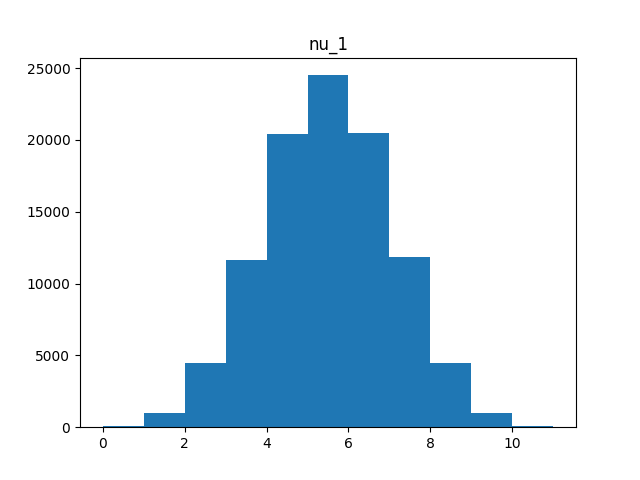
\includegraphics[scale=0.8]{nu_1.png}\\
		Counts of $\nu_{rand}$: [95, 924, 4431, 11639, 20450, 24727, 20582, 11554, 4439, 1046, 113]\\
		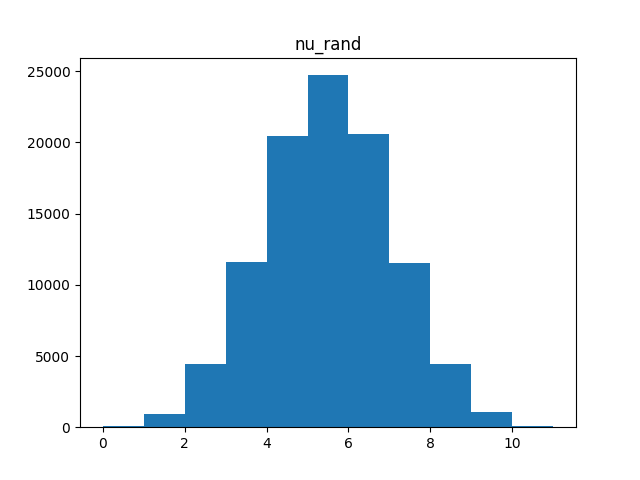
\includegraphics[scale=0.8]{nu_rand.png}\\
		Counts of $\nu_{min}$: [62487, 37510, 3, 0, 0, 0, 0, 0, 0, 0, 0]\\
		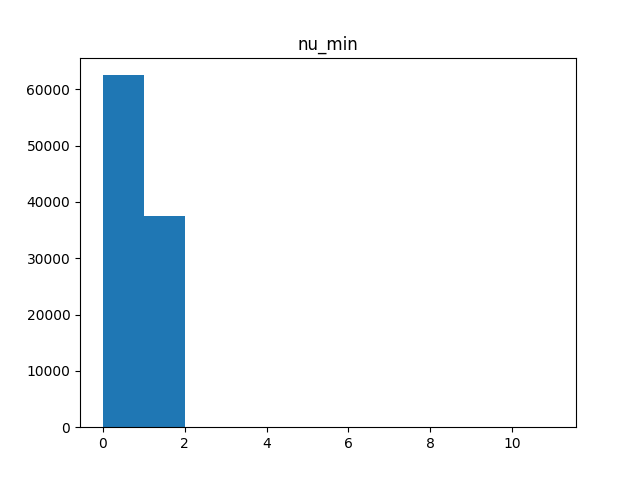
\includegraphics[scale=0.8]{nu_min.png}
	\subsection*{(c)}
		Note: the following plots were supposed to look like the hand-drawn one for the last question but I don't know how to plot step functions in python. Each line segment is supposed to stay flat starting on the left point. If you get the idea please don't take off points. Thanks.\\
		For $c_1$:\\
		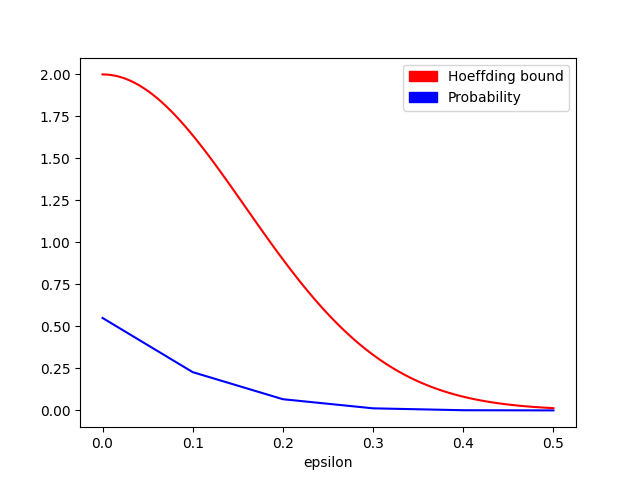
\includegraphics[scale=0.8]{epsilon_1.png}\\
		For $c_{rand}$:\\
		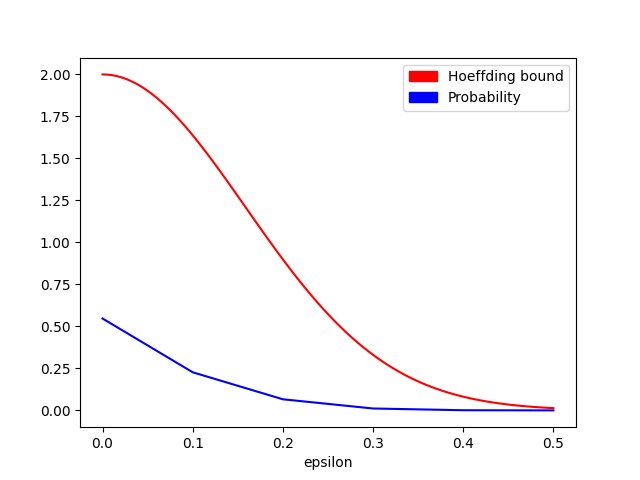
\includegraphics[scale=0.8]{epsilon_rand.png}\\
		For $c_{min}$:\\
		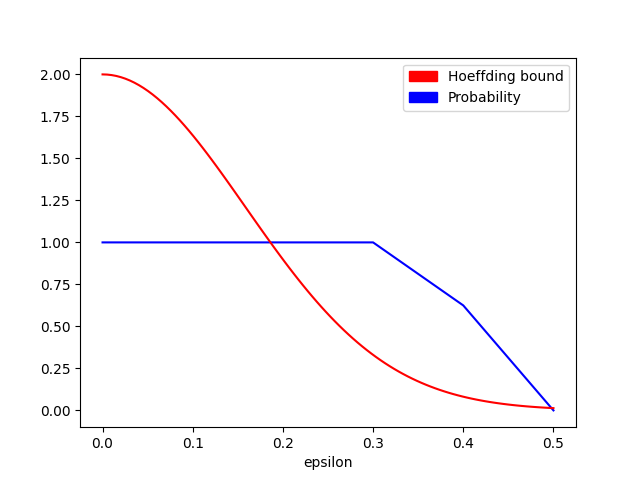
\includegraphics[scale=0.8]{epsilon_min.png}
	\subsection*{(d)}
		$c_1$ and $c_{rand}$ obey the Hoeffding bound and $c_{min}$ does not because for $c_1$ and $c_{rand}$ the probability curve is always below the Hoeffding bound curve. This is not true for $c_{min}$.
	\subsection*{(e)}
		$c_1$ and $c_{rand}$ are selected from the bin of all the 1000 coins while $c_{min}$ is selected from the bin of coins with minimum number of heads.
		
	\section*{Exercise 1.11}
	\subsection*{(a)}
		No because we can never draw conclusion outside the data for sure.
		
	\subsection*{(b)}
		Yes for the same reason above.
		
	\subsection*{(c)}
		\begin{align*}
			P(\text{more +1's than -1's in }D) = \sum\limits_{n = 13}^{25}{25 \choose n}\times 0.9^n \times 0.1^{25 - n} \approx \boxed{1}
		\end{align*}
		
	\subsection*{(d)}
		No because $D$ is a random sample, whose expected frequency of +1's always equals $p$. The hypothesis produced by S will therefore always be more likely to agree with inputs out of $D$.
		
	\section*{Exercise 1.12}
		The best I can promise is (c) because in machine learning it's always possible to fail.
		
	\section*{Problem 1.3}
	\subsection*{(a)}
		Given that $\mathbf w^*$ separates the data, we can conclude that $\forall n: y_n = sign(\mathbf w^{*T}\mathbf x_n)$.\\
		Therefore, $\forall n: y_n(\mathbf w^{*T}\mathbf x_n) > 0$, which means $\min_n y_n(\mathbf w^{*T}\mathbf x_n) > 0$.
		
	\subsection*{(b)}
		%Since $\rho > 0$ and $y_n \in {+1, -1}$, $\rho = min_n |\mathbf w^{*T}\mathbf x_n|$\\
		\begin{align*}
			\mathbf w^T(t)\mathbf w^* &= (\mathbf w^T(t-1) + y_i\mathbf x^T_i)\mathbf w^*\text{ for some }i\\
			&= \mathbf w^T(t-1)\mathbf w^* + y_i\mathbf x^T_i\mathbf w^*\\
			&\geq \mathbf w^T(t-1)\mathbf w^* + \min_i y_i\mathbf x^T_i\mathbf w^*\\
			&= \mathbf w^T(t-1)\mathbf w^* + \rho
		\end{align*}
		Proof of $\mathbf w^T(t)\mathbf w^* \geq t\rho$ by Induction:\\
		Base Case $t = 0$:
		\begin{align*}
			\mathbf w^T(0)\mathbf w^* = 0 \geq 0\rho = 0
		\end{align*}
		Inductive Step:\\
		Assume $\mathbf w^T(t)\mathbf w^* \geq t\rho$
		\begin{align*}
			\mathbf w^T(t+1)\mathbf w^* &\geq \mathbf w^T(t)\mathbf w^* + \rho\\
			&\geq t\rho + \rho\\
			&= (t+1)\rho
		\end{align*}
		
	\subsection*{(c)}
		\begin{align*}
			\text{Given } \mathbf w(t) &= \mathbf w(t-1) + y(t-1)\mathbf x(t-1)\\
			||\mathbf w(t)||^2 &= ||\mathbf w(t-1)||^2 + 2y(t-1)\mathbf w^T(t-1)\mathbf x(t-1) + y^2(t-1)||\mathbf x(t-1)||^2\\
			\text{Knowing } &y(t-1)\mathbf w^T(t-1)\mathbf x(t-1) \leq 0\\
			||\mathbf w(t)||^2 &\leq ||\mathbf w(t-1)||^2 + y^2(t-1)||\mathbf x(t-1)||^2\\
			&= ||\mathbf w(t-1)||^2 + ||\mathbf x(t-1)||^2
		\end{align*}
		
	\subsection*{(d)}
		Base Case $t = 0$:
		\begin{align*}
			||\mathbf w(0)||^2 = ||\mathbf 0||^2 = 0 \geq 0R^2 = 0
		\end{align*}
		Inductive Step:
		\begin{align*}
			\text{Assume } ||\mathbf w(t)||^2 &\leq tR^2\\
			||\mathbf w(t+1)||^2 &\leq ||\mathbf w(t)||^2 + ||\mathbf x(t)||^2\\
			&\leq tR^2 + (\max_n ||\mathbf x_n||)^2\\
			&= tR^2 + R^2\\
			&= (t+1)R^2
		\end{align*}
		
	\section*{(e)}
		\begin{align*}
			\text{From part (b): } \mathbf w(t)\mathbf w^* \geq t\rho\\
			\text{From part (d): } ||\mathbf w(t)||^2 \leq tR^2\\
			||\mathbf w(t)|| \leq R\sqrt t\\
			\frac{ \mathbf w^T(t)\mathbf w^* }{||\mathbf w(t)||} &\geq \frac{t\rho}{R\sqrt t}\\
			&= \frac{\rho} R \sqrt t\\
			\text{Cauchy-Shwartz Inequality: }\mathbf w^T(t)\mathbf w^* &\leq ||\mathbf w(t)||\ ||\mathbf w^*||\\
			\frac{\mathbf w^T(t)\mathbf w^* }{ ||\mathbf w(t)||} &\leq ||\mathbf w^*||\\
			\frac{\rho} R \sqrt t &\leq ||\mathbf w^*||\\
			t &\leq \frac{R^2||\mathbf w^*||^2}{\rho^2}
		\end{align*}
		
	\section*{Problem 1.7}
	\subsection*{(a)}
		$\mu = 0.05$:
		\begin{align*}
			P(\text{single coin has } \nu > 0) &= 1 - {10 \choose 0}\times (1 - 0.05)^{10}\\
			&\approx 0.401\\
			P(\text{some coin has } \nu = 0) &= 1 - P(\text{all coins have } \nu > 0)\\
			\text{For 1 coin: }P(\text{some coin has } \nu = 0) &\approx 1 - 0.401\\
			&= \boxed{0.599}\\
			\text{For 1000 coins: } P(\text{some coin has } \nu = 0) &\approx 1 - 0.401^{1000}\\
			&\approx \boxed{1}\\
			\text{For 1000000 coins: } P(\text{some coin has } \nu = 0) &\approx 1 - 0.401^{1000000}\\
			&\approx \boxed{1}\\
		\end{align*}
		$\mu = 0.8$:
		\begin{align*}
			P(\text{single coin has } \nu > 0) &= 1 - {10 \choose 0}\times (1 - 0.8)^{10}\\
			&\approx 0.99999990\\
			P(\text{some coin has } \nu = 0) &= 1 - P(\text{all coins have } \nu > 0)\\
			\text{For 1 coin: }P(\text{some coin has } \nu = 0) &\approx 1 - 0.99999990\\
			&\approx \boxed{0}\\
			\text{For 1000 coins: } P(\text{some coin has } \nu = 0) &\approx 1 - 0.99999990^{1000}\\
			&\approx \boxed{1.02\times 10^{-4}}\\
			\text{For 1000000 coins: } P(\text{some coin has } \nu = 0) &\approx 1 - 0.99999990^{1000000}\\
			&\approx \boxed{9.73 \times 10^{-2}}\\
		\end{align*}
	\subsection*{(b)}
		\begin{align*}
			N = 6 &\implies \nu \in \{0, \frac16, \frac13, \frac12, \frac23, \frac56, 1\}\\
			P(\max\limits_i|\nu_i - \mu_i| > \epsilon) &= 1 - P(|\nu_1 - \mu_1| \leq \epsilon)P(|\nu_2 - \mu_2| \leq \epsilon)\\
			P(\max\limits_i|\nu_i - \mu_i| > 0) &= 1 - P(\nu_1 = \frac12)P(\nu_2 = \frac12)\\
			&= 1 - ({6 \choose 3}(\frac12)^6)^2\\
			&\approx 0.902\\
			P(\max\limits_i|\nu_i - \mu_i| > \frac16) &= 1 - P(\nu_1 \in \{\frac13, \frac12, \frac23\})P(\nu_2 \in \{\frac13, \frac12, \frac23\})\\
			&= 1 - ({6\choose 2}(\frac12)^6 + {6 \choose 3}(\frac12)^6 + {6 \choose 4}(\frac12)^6)^2\\
			&\approx 0.390\\
			P(\max\limits_i|\nu_i - \mu_i| > \frac13) &= 1 - P(\nu_1 \in \{\frac16, \frac13, \frac12, \frac23, \frac56\})P(\nu_2 \in \{\frac16, \frac13, \frac12, \frac23, \frac56\})\\
			&= 1 - (({6 \choose 1} + {6\choose 2} + {6 \choose 3} + {6 \choose 4} + {6 \choose 5})(\frac12)^6)^2\\
			&\approx 0.062\\
			P(\max\limits_i|\nu_i - \mu_i| > \frac12) &= 0
		\end{align*}
		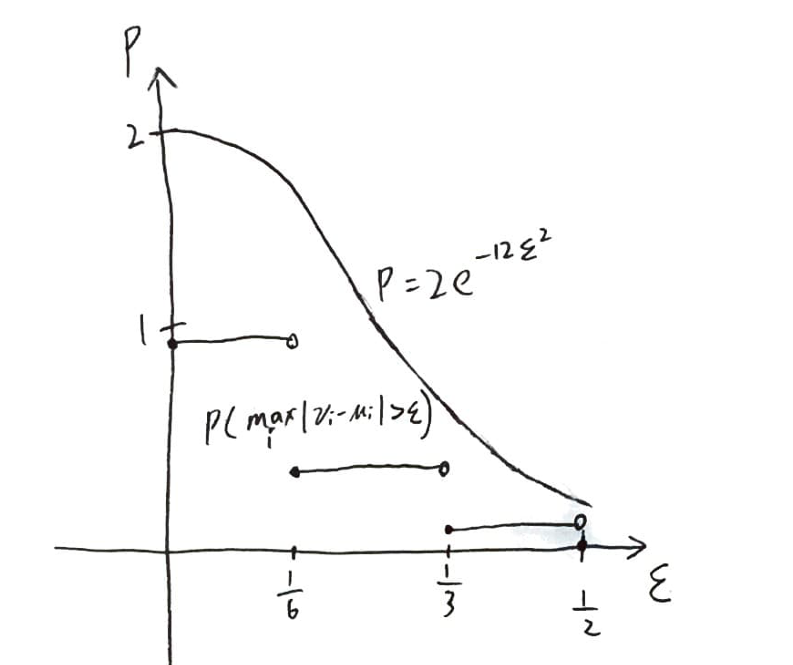
\includegraphics[scale=0.4]{p1.7b.png}
\end{document}